\subsection{Repérage}

\begin{mydef}
	\iftoggle{eleve}{%
		Sur une droite graduée, \hrulefill
		
		\vspace*{0.2cm}
		\hrulefill
	}{%
		Sur une droite graduée, chaque point est repéré par un nombre relatif, son \kw{abscisse}.
}
\end{mydef}


\begin{myex}
	\begin{center}
		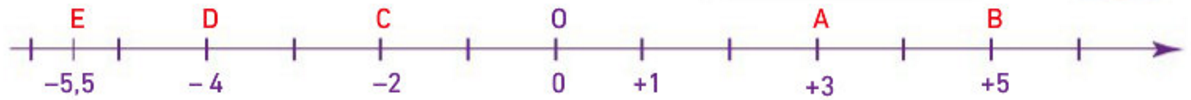
\includegraphics[scale=0.5]{img/droite2}		
	\end{center}

	\begin{multicols}{2}
		\begin{itemize}
			\iftoggle{eleve}{%
				\item L'abscisse du point A est 
				\item L'abscisse du point B est 
				\item L'abscisse du point C est 
				\item L'abscisse du point D est 
				\item L'abscisse du point E est 
				\item L'abscisse du point O est 
			}{%
				\item L'abscisse du point A est +3;
				\item L'abscisse du point B est +5;
				\item L'abscisse du point C est -2;
				\item L'abscisse du point D est -4.
				\item L'abscisse du point E est \num{-5.5};
				\item L'abscisse du point O est 0;
			}
		\end{itemize}
	\end{multicols}
\end{myex}


\begin{mydefs}
	\begin{itemize}
		\iftoggle{eleve}{%
			\item Un repère orthogonal est formé par \hrulefill
			
			\vspace*{0.2cm}
			\hrulefill
			
			\vspace*{0.2cm}
			\hrulefill
			
			\vspace*{0.2cm}
			\hrulefill
			
			\vspace*{0.2cm}
			\hrulefill
			
			\item Un point du plan est repéré par \hrulefill
			
			\vspace*{0.2cm}
			\hrulefill
			
			\vspace*{0.2cm}
			\hrulefill
			
			\vspace*{0.2cm}
			\hrulefill
			
			\vspace*{0.2cm}
			\hrulefill
		}{%
		\item Un repère orthogonal est formé par deux droites graduées perpendiculaires et de même origine. La droite horizontale est l'\kw{axe des abscisses}, la verticale est l'\kw{axe des ordonnées}.
		
		\item Un point du plan est repéré par deux nombres relatifs, ses \kw{coordonnées}. Le premier nombre est son \kw{abscisse}, le second son \kw{ordonnée}. On note ces coordonnées $(abscisse \: ; \: ordonnée)$.
	}
	\end{itemize}
\end{mydefs}


\begin{myexs}
	
		\begin{center}
			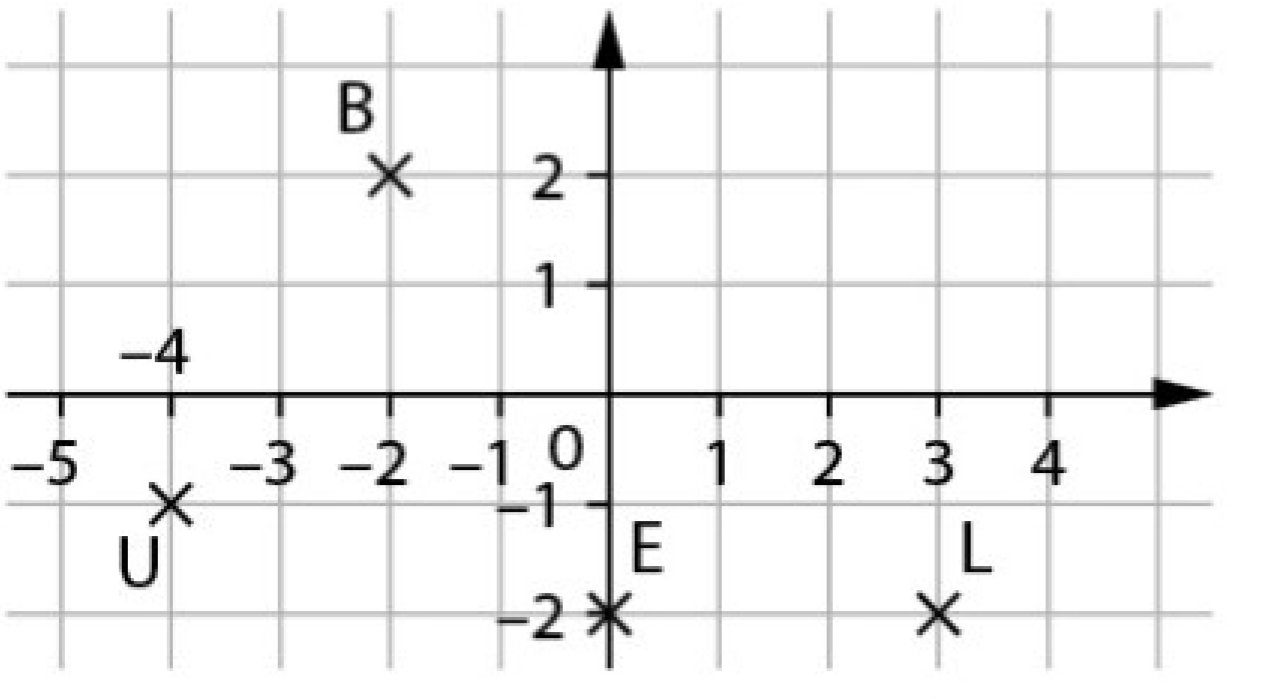
\includegraphics[scale=0.4]{repere}
		\end{center}
	

	\begin{itemize}
		\iftoggle{eleve}{%
			\item L'abscisse du point $A$ est \hrulefill
			
			\vspace*{0.2cm}
			\hrulefill
			
			\item L'abscisse du point $B$ est \hrulefill
			
			\vspace*{0.2cm}
			\hrulefill
		}{%
		\item L'abscisse du point $A$ est +3, son ordonnée est +2, ses coordonnées sont $(+3; +2)$.
		
		\item L'abscisse du point $B$ est +1, son ordonnée est -2, ses coordonnées sont $(+1; -2)$.
	}
	\end{itemize}

\end{myexs}



\subsection{Comparaison}

\begin{myprops}
	Pour comparer deux nombres relatifs :
	\begin{itemize}
		\iftoggle{eleve}{%
			\item Si les deux nombres sont \hrulefill

			\vspace*{0.2cm}
			\hrulefill

			\item Si les deux nombres sont \hrulefill 
			
			\vspace*{0.2cm}
			\hrulefill
			
			\item Si les deux nombres sont \hrulefill
			
			\vspace*{0.2cm}
			\hrulefill
		}{%
			\item Si les deux \kw{nombres sont positifs}, le plus grand est celui qui a la \kw{plus grande distance à zéro};
			\item Si les deux nombres sont de \kw{signes différents}, le plus grand est le \kw{nombre positif};
			\item Si les deux \kw{nombres sont négatifs}, le plus grand est celui qui a la \kw{plus petite distance à zéro};
		}
	\end{itemize}
\end{myprops}


\begin{myexs}
	\begin{center}
		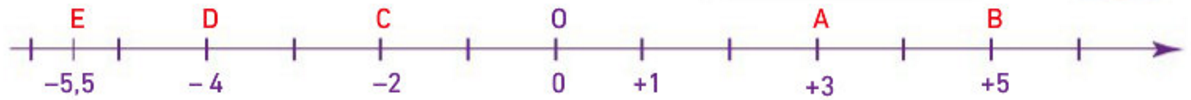
\includegraphics[scale=0.5]{img/droite2}		
	\end{center}


	\begin{multicols}{2}
		\begin{itemize}
			\iftoggle{eleve}{%
				\item +5 \hspace*{1cm}  +3 (car \hrulefill
				\item +5 \hspace*{1cm} +1 (car \hrulefill
				\item +1 \hspace*{1cm} \num{-2} (car \hrulefill
				\item +5 \hspace*{1cm} \num{-4} (car \hrulefill
				\item \num{-4} \hspace*{1cm} \num{-5.5} (car \hrulefill
				\item \num{-2} \hspace*{1cm} \num{-5.5} (car \hrulefill
			}{%
				\item +5 > +3 (car 5 > 3)
				\item +5 > +1 (car 5 > 1)
				\item +1 > \num{-2} (car +1 est positif)
				\item +5 > \num{-4} (car +5 est positif)
				\item \num{-4} > \num{-5.5} (car 4 < \num{5.5})
				\item \num{-2} > \num{-5.5} (car 2 < \num{5.5})
			}
		\end{itemize}
	\end{multicols}
\end{myexs}